\section{Аналитический раздел}
\subsection{Постановка задачи}
В соответствии с заданием на курсовую работу по дисциплине <<Операционные системы>> требуется разработать ПО, позволяющее задавать определённые действия системы движением нескольких пальцев по тачпаду.

Для выполнения задания требуется решить следующие задачи:
\begin{enumerate}
	\item провести анализ существующих подходов к обработке устройств ввода;
	\item провести анализ существующих способов задания действий движением нескольких пальцев по тачпаду;
	\item провести анализ возможности исполнения системой заданных действий;
	\item разработать алгоритмы, необходимые для реализации ПО;
	\item разработать ПО, предоставляющее требуемую функциональность;
	\item провести исследование разработанного ПО.
\end{enumerate}

Для разработки и тестирования данной работы используется портативный компьютер \texttt{Huawei Matebook X Pro} и операционная система \texttt{Linux} с дистрибутивом \texttt{Kali Linux}.

\subsection{Загружаемый модуль ядра}

Ядро Linux относится к классу монолитных. В архитектуре данного класса прикладные приложения выполняются посредством создания отдельной ветки кода в пространстве ядра. Поскольку в ранних версиях расширение функциональности требовало перекомпиляции ядра, что было недопустимо для систем промышленного уровня, позднее была добавлена технология модуля ядра. Модуль ядра может реализовывать драйвер устройства, файловую систему или сетевой протокол

К преимуществам такого подхода следует отнести сокращение неиспользуемого кода в базовом ядре и, как следствие, уменьшение занимаемой памяти. Недостатком является фрагментация ядра, после загрузки
модулей, несмотря на то, что код базового ядра не фрагментируем. Фрагментация ведет к незначительному снижению производительности из-за
увеличения пропусков записей TLB. Также использование загружаемого модуля снижает безопасность системы, поскольку злоумышленники, имея
доступ в пространство ядра, могут скрывать процессы и файлы.

\subsubsection{Драйвера}

В современных ядрах \texttt{Linux} изменение функциональности внешних устройств возможно с помощью драйверов верхнего уровня, представляющих собой загружаемые модули ядра. Драйверы полностью скрывают детали, касающиеся работы устройства и предоставляют чёткий программный интерфейс для работы с аппаратурой. В \texttt{Linux} имеется три типа драйверов:

\begin{enumerate}
	\item драйверы первого типа являются частью программного кода ядра. Соответствующие устройства автоматически обнаруживаются системой и
	становятся доступны доя приложений;
	
	\item драйверы второго типа представлены загружаемыми модулями ядра. Они	оформлены в виде отдельных файлов. Для их подключения необходимо выполнить команду подключения модуля. Если необходимости в
	использовании нет, модуль можно выгрузить из памяти. Использование
	модулей обеспечивает большую гибкость, так как каждый драйвер может быть переконфигурирован без остановки системы;
	
	\item в драйверах третьего типа программный код драйвера поделён между ядром и специальной утилитой, предназначенной для управления данным устройством.
\end{enumerate}

Во всех драйверах взаимодействие с устройством осуществляет ядро или
модуль ядра, а пользовательские программы взаимодействуют через специальные файлы, расположенные в каталоге \texttt{/dev} и его подкаталогах.

\subsubsection{Обработчик устройства ввода}

Драйвер интерактивного устройства ввода -- это модуль, обеспечивающий возможность взаимодействия с устройством через прерывания.

Алгоритм регистрации обработчика прерывания устройства ввода \cite{docs} может быть представлен в виде следующей последовательности действий: 
\begin{enumerate}
	\item заполнение структуры \texttt{struct input\_handler};
	\item регистрация обработчика функцией \texttt{input\_register\_handler}. 
\end{enumerate}

\subsection{Передача информации из пространства ядра в пространство пользователя}

В файловой системе (ФС) \texttt{proc} можно создавать свои файлы, ссылки, директории. Структура \texttt{proc\_dir\_entry}, определённая в файле \texttt{<fs/proc/internal.h>}. Для определения обратных вызовов чтения и записи предоставляется структура \texttt{proc\_ops}. Данная структура определена в файле
\texttt{<include/linux/proc\_fs.h>}, наиболее важные поля которой представлены в листинге \ref{lst:procops}.

\begin{lstlisting}[label=lst:procops,caption=Структура proc\_ops, language=c]
struct proc_ops {
	unsigned int proc_flags;
	int	(*proc_open)(struct inode *, struct file *);
	ssize_t	(*proc_read)(struct file *, char __user *, size_t, loff_t *);
	...
	ssize_t	(*proc_write)(struct file *, const char __user *, size_t, loff_t *);
	...
	int	(*proc_release)(struct inode *, struct file *);
	...
} __randomize_layout;
\end{lstlisting}

Использование функций \texttt{proc\_create} и \texttt{remove\_proc\_entry}, определённых в файле \texttt{<include/linux/proc\_fs.h>}, позволяет регистрировать и отменять регистрацию файла в \texttt{proc}. Для взаимодействия ядра с приложениями используется функция \texttt{copy\_to\_user}, определение которой представлено в файле \texttt{<include/linux/uaccess.h>}. Данная функция копирует блоки данных из ядра в пространство пользователя. Для передачи информации в пространство ядра используется функция \texttt{copy\_from\_user}.

\subsection{Прерывания}

Прерывания делятся на:
\begin{itemize}
	\item исключения (деление на ноль, переполнение стека), синхронные;
	\item системные вызовы (программные) - вызываются с помощью соответствующей команды из программы (\texttt{int 21h}), синхронные;
	\item аппаратные прерывания (прерывания от системного таймера, клавиатуры), асинхронные. 
\end{itemize}

Прерывания делятся на 2 группы:

\begin{itemize}
	\item быстрые;
	\item медленные. 
\end{itemize}

Для того чтобы сократить время обработки медленных прерываний, они делятся на 2 части:

\begin{itemize}
	\item \texttt{top half}, верхняя половина, запускается в результате получения процессором сигнала прерывания;
	\item \texttt{bottom half}, нижняя половина, отложенные вызовы.
\end{itemize}

\subsection{Запуск процессов пользователя из пространства ядра}

\subsubsection{call\_usermodehelper}

Использование функции \texttt{call\_usermodhelper} \cite{src} позволяет выполнять процесс пользователя из пространства ядра. Работа этой функции аналогична работе вызова \texttt{exec()} в пространстве пользователя. Особенность данного метода заключается в том, что процесс запускается без управляющего терминала и с нестандартным окружением. Внутренняя реализация функции представлена на рисунке \ref{fig:umh}.

\begin{figure}[h!btp]
	\centering
	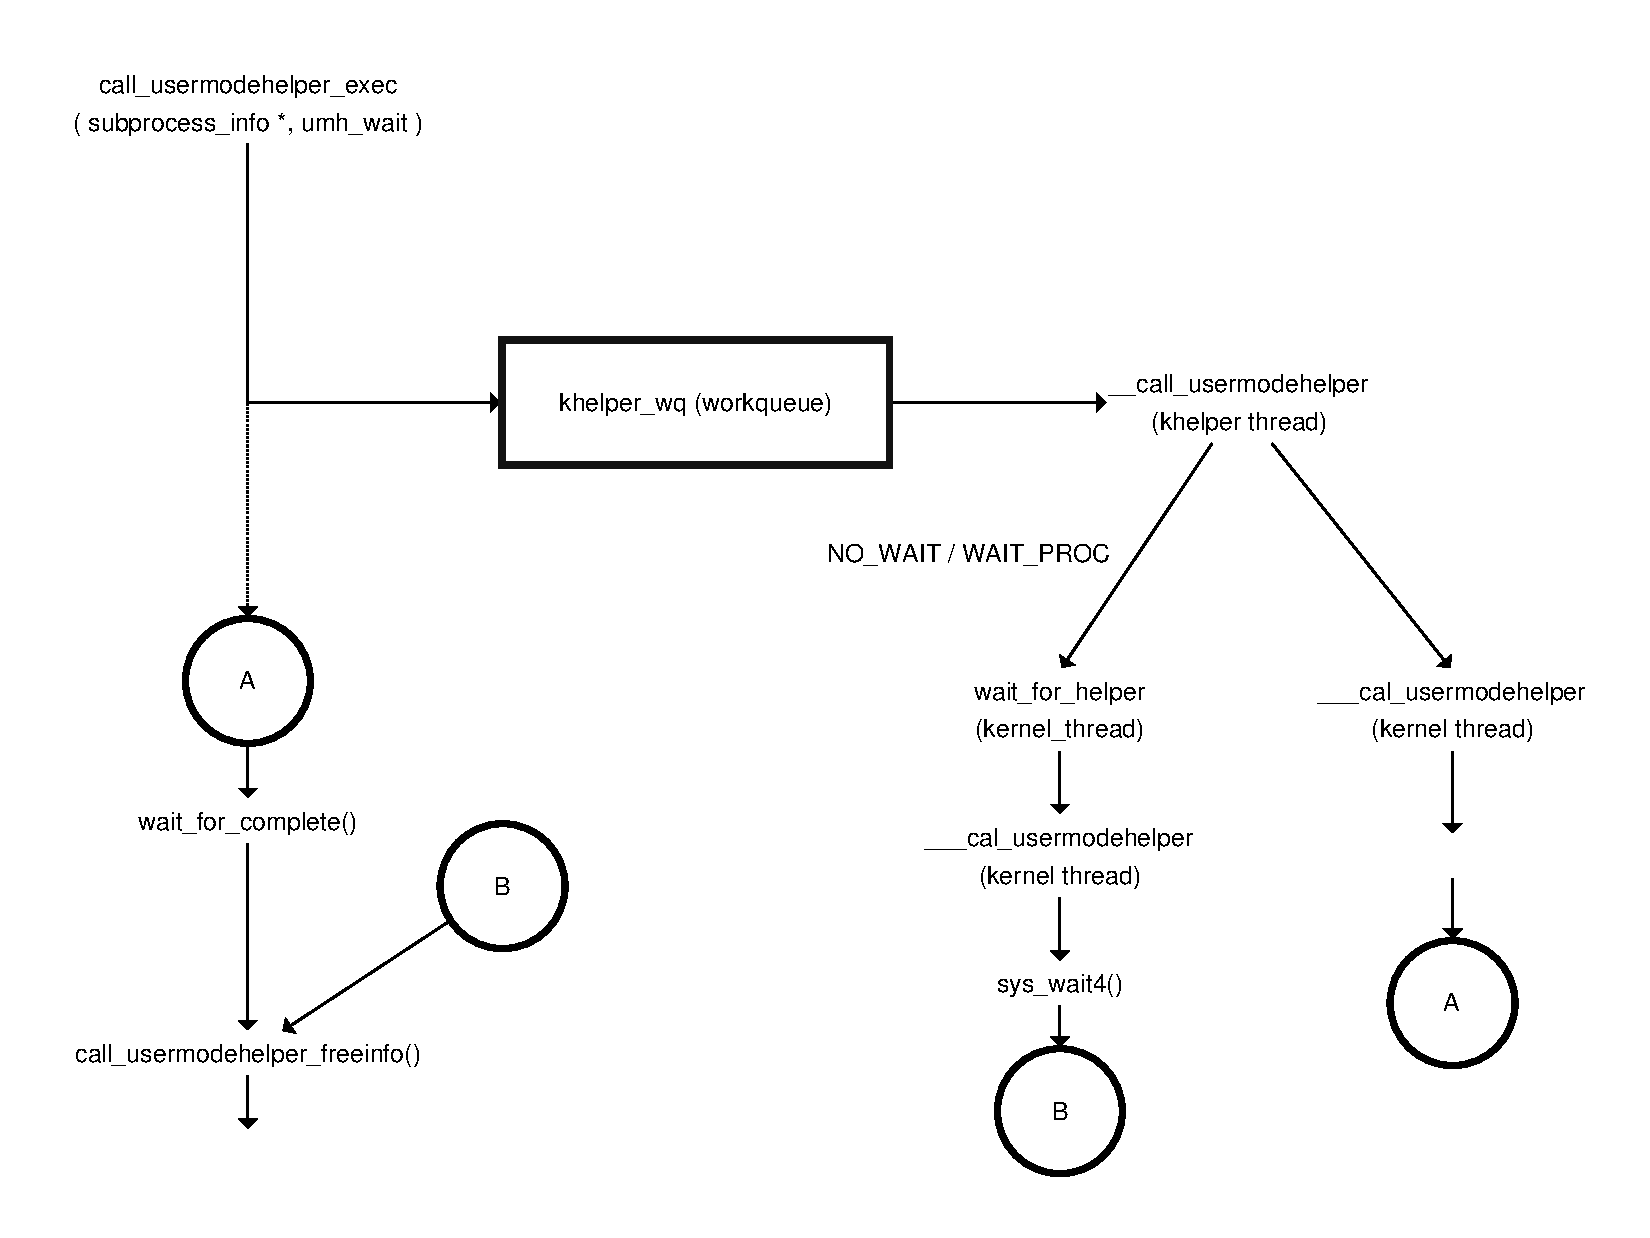
\includegraphics[width=0.9\textwidth]{inc/usermodehelper.pdf}
	\caption{Внутренняя реализация функции \texttt{call\_usermodehelper}}
	\label{fig:umh}	
\end{figure}

\subsubsection{Планировщик ядра}

Для выполнения процесса в пространстве пользователя необходимо вызвать функцию \texttt{call\_usermodehelper} с флагом ожидания \texttt{UMH\_WAIT\_PROC}. В таком случае мы будем ожидать завершение процесса. В контексте обработчика устройства ввода это невозможно, обработчик находится в неделимом контексте, который не допускает ожидание.

Для это можно воспользоваться общей очередью работ ядра. При планировании работы общим планировщиком ядра, системой создаётся отдельный поток, в котором будет выполнена работа. В таком случае ожидание возможно и процесс будет выполнен.

Потоки ядра используются для выполнения асинхронного ввода-вывода. Ядро создаёт поток для обработки запросов каждой такой операции. Потоки также могут быть использованы для обработки прерываний.

\subsubsection{Переключение потоков}

Переключение потоков является основной задачей планировщика. В ОС Linux механизм планирования основывается на приоритетах. Когда процесс просыпается, ядро устанавливает значение текущего приоритета, равное значению приоритета сна события или ресурса, на котором он был заблокирован. Такой процесс будет назначен на выполнение раньше, чем другие процессы в режиме задачи.

Когда процесс завершил выполнение системного вызова и находится в состоянии возврата в режим задачи, его приоритет сбрасывается обратно в значение текущего приоритета в режиме задачи.

\subsection{Multi Touch протокол}

Для определения движения нескольких пальцев по тачпаду следует воспользоваться \texttt{Multi Touch} протоколом. Для каждого пальца отправляется набор событий, содержащий: 

\begin{itemize}
	\item \texttt{ABS\_MT\_SLOT} -- порядковый номер;
	\item \texttt{ABS\_MT\_TRACKING\_ID} -- идентификатор;
	\item \texttt{ABS\_MT\_POSITION\_X} -- координата X;
	\item \texttt{ABS\_MT\_POSITION\_Y} -- координата Y.
\end{itemize}

Каждый набор событий завершается событием \texttt{SYN\_REPORT}. 

При удалении пальца с тачпада идентификатор \texttt{ABS\_MT\_TRACKING\_ID} для соответствующего пальца будет равен -1. Пример потока событий для двух пальцев показан в листинге \ref{lst:mt2}.

\begin{lstlisting}[language=c, label=lst:mt2, caption={Поток событий для двух пальцев}]
	ABS_MT_SLOT 0
	ABS_MT_TRACKING_ID 45
	ABS_MT_POSITION_X x[0]
	ABS_MT_POSITION_Y y[0]
	ABS_MT_SLOT 1
	ABS_MT_TRACKING_ID 46
	ABS_MT_POSITION_X x[1]
	ABS_MT_POSITION_Y y[1]
	SYN_REPORT
\end{lstlisting}

\subsection{Выводы}

В результате проведённого анализа было заключено следующее:
\begin{enumerate}
	\item реализовать алгоритм определения шаблона;
	\item для выполнения заданных действий использовать общую очередь работ;
	\item реализовать обработчик устройства ввода в виде загружаемого модуля ядра;
	\item для задания действий системы воспользоваться скриптовым языком \texttt{bash};
	\item для передачи конфигурации в загружаемый модуль использовать виртуальную файловую систему \texttt{/proc/}.
\end{enumerate}

\clearpage